\chapter{Interoperability and Automated Tests: DevOps}
\label{ch:devops}

Previous chapters introduced different tools and approaches for modelling norm-governed cyber-infrastructures, however, what typically holds such approaches back for real world applications is usability and adoptability for designers and models. Development solutions, such as testing and integration, undeniably play a central role in the daily practice of software engineering, and this explains why better and more efficient libraries and services are continuously made available to developers and designers. Could the MAS developers community similarly benefit from utilizing state-of-the-art testing approaches? The chapter investigates the possibility of bringing  modern software testing and integration tools as those used in mainstream software engineering into multi-agent systems engineering. Our contribution explores and illustrates, by means of a concrete example, the possible interactions between the agent-based programming framework ASC2 (AgentScript Cross-Compiler)  and various testing approaches (unit/agent testing, integration/system testing, continuous integration) and elaborate on how the design choices of ASC2 enable these interactions.


\section{Introduction}

Software testing is attracting increased interest in industry \cite{market_reports_2019} and it is one of the most used methods of software verification. One of the reasons of this success lies in the advancement and popularization in the software engineering community of methodologies commonly known as \textit{DevOps}, in particular of techniques of automated testing in \textit{continuous integration} (CI). Generally, CI refers to the facilitation provided by third-party tools for automating the build/test process of a software. In recent years, online DevOps services such as TravisCI\footnote{\url{https://travis-ci.com/}} and CircleCI\footnote{\url{https://circleci.com/}} have been increasingly used by software engineers to improve the efficiency of their testing process, a practice which plausibly resulted in increased quality of the developed software.

Very recently, Fisher et al. \cite{Fisher2020} have suggested that testing approaches would be an important complement to formal approaches to MAS verification, if they could be automated and integrated in a seamless way into MAS development. In our view, seamless integration  does not mean only that agent programmers are able to use the vast amount of software testing tools available to mainstream languages like Java or Python, but, more importantly, that they are also able to use (almost) language- and framework- agnostic online services as those used for CI. This chapter explores this idea, aiming to illustrate what the MAS community could gain by using industry standard testing tools and discussing what would be the theoretical and practical trade-offs for this choice. We investigate possible interactions of testing with agent-based programming, and its relation with other verification techniques. More concretely, we demonstrate various approaches to enhance the productivity of MAS development cycle in the ASC2 framework via mainstream software testing and integration tools, and elaborate on the design choices of ASC2 that affect the testability of agent-programs with the mentioned tools. Then, we explore on how this approach can be generalized for other MAS frameworks.

The motivation for this chapter arises from research conducted
% This work is motivated by the applied research
%domain focuses 
on data-sharing infrastructures (e.g. data marketplaces). At functional level, a data-sharing application corresponds to a coordination of several computational actors distributed over multi-domain networks. Those actors generally include certifiers, auditors, and other actors having monitoring and enforcement roles, ensuring some level of security and trustworthiness on data processing \cite{Zhou2020}.  Typically distributed across several jurisdictions, networks may be subjected to distinct norms and policies, to be added to  various infrastructural policies provided at domain level and \textit{ad-hoc} policies set up by the users. Some of these norms, as for instance the GDPR, bind  processing to conditions and specific purposes, but, more in general, all compliance checking on social systems requires to know and to infer (in case of a failure on expectations) \textit{why} an actor is performing certain operations. 
% As this example shows, regulating these infrastructures requires reproducing to a certain extent constructs similar to those observed in human reasoning (e.g. For which purpose is the agent asking access to the resource? On which basis is the infrastructure granting access?). For traceability and explainability reasons, decisions concerning actions need to be processed by the infrastructure as much as relevant operational aspects. 
Agent-based programming, and particularly the Belief-Desire-Intention (BDI) model, by looking at computational agents as \textit{intentional agents}, provides the ``purpose'' level of abstraction available by design, and for this reason it is a natural technological candidate for this application domain. 

The BDI model been extensively investigated as basis to represent computational agents that exhibit rational behaviour \cite{Herzig2017}.
%and multiple programming languages and frameworks have been introduced based on it, as AgentSpeak(L)/Jason \cite{RaoAS1996,Bordini2005}, 3APL/2APL \cite{Dastani2APL}, and GOAL \cite{Hindriks2009a}.
Recent works as e.g. \cite{Kampik2020} investigated various issues holding when mapping logic-oriented agent-based programs into an operational setting. In contrast, this chapter focuses instead on the \textit{development practice} aspect: as soon as we attempted to program data-sharing applications as agents, we experienced the lack of  mature software engineering toolboxes, thus hindering a continuous integration with the infrastructural-level components developed in parallel by our colleagues.

%Agent-based programming, and in particular the Belief-Desire-Intention (BDI) model by looking at computational agents as \textit{intentional agents}, provides this level of abstraction available by design, and for this reason, it is in principle a serious technological candidate for this application domain.  Recent works as e.g. \cite{Kampik2020,MohajeriParizi2020} investigated various issues holding when mapping logic-oriented agent-based programs into an operational setting. This chapter focuses instead on the \textit{development practice} aspect: as soon as we attempted to program data-sharing applications as agents, we experienced the lack of  mature software engineering toolboxes, thus hindering a continuous integration with the infrastructural-level components developed in parallel by our colleagues.

The document proceeds as follows: section \ref{sec:back} provides a background and related works on verification of MAS, in section \ref{sec:approach} we introduce our approach on MAS testing in ASC2 framework with mainstream tools. An illustrative example of this approach is presented in section \ref{sec:example}. Finally, section \ref{sec:discussion} provides the discussion and comments on possible extensions and future developments.

% a possible approach allowing seamless integration of modern software testing tools and services with agent-based and multi-agent systems programming.
% Furthermore this work presents an approach for seamless integration of modern software testing tools and services into both agent-based programming and multi-agent systems.



%Software testing is a series of processes, designed to make sure a computational entity does what it was designed to do and it does not do anything unintended. Testing allows the development teams to have some degree of assurance about the behaviors of different pieces of their product \cite{ArtOfTesting}.

% Furthermore, now that intelligent and autonomous systems are becoming more integrated in everyday life of humans, practical approaches for verification of such systems also become more crucial \cite{Fisher2020}. 
%Software testing is typically integrated as part of the development cycle which means it can be done in a iterative and agile manner and for many applications it can efficiently provide a sufficient level of assurance for the development team \cite{Fisher2020}.

\section{Verification of 
(Multi-)Agent Systems}
\label{sec:back}
% \begin{comment} % I would put that in another point
% \subsection{Belief-Desire-Intention (BDI) Model}

% At the agent level, in this chapter we  specifically explore testing of agents specified in the the \textit{belief-desire-intention} (BDI) model of agency. Having its roots in a theory of mind \cite{bratman1987intention}, and so referring to categories that are used typically to address human behaviour to describe agents, the BDI model \cite{Rao1995} has been extensively investigated as basis to represent computational agents that exhibit rational behaviour \cite{Herzig2017}. 
% % uses taxonomies that are used typically to address human behaviour to describe agents.
% \textit{Beliefs} are the factual (and possibly inferential) information the agent has about itself and its environment. \textit{Desires}, in their simplest form, are objectives the agent wants to accomplish. % \Gio{(i.e. facts desired to be true)}.
% %in the environment. 
% \textit{Intentions} are the courses of action the agent has committed to. In practice, BDI agents include concepts of \textit{Goals} and \textit{Plans}. Goals are instantiated desires % associated to reactive behaviors to certain events 
% and plans are abstract specifications relating a goal to the means of achieving that goal (intentions become commitment towards plans). Multiple programming languages and frameworks have been introduced based on the BDI model, as AgentSpeak(L)/Jason \cite{RaoAS1996,Bordini2005}, 3APL/2APL \cite{Dastani2APL}, GOAL \cite{Hindriks2009a}.
% \end{comment}



Verification is a crucial phase in any software (and system) development process, and as such it has been  addressed also by the Multi-Agent Systems (MAS) community. The survey presented in \cite{Bakar2018} provides an empirical review of over 230 works related to verification of MAS. 

At higher level,  approaches for the verification of autonomous systems fall into five categories \cite{Fisher2020}: (a) \textit{model checking}, (b) \textit{theorem proving}, (c) \textit{static analysis}, (d) \textit{run-time verification}, and (e) \textit{(systematic) testing}. While the first four approaches (a-d) are considered formal or at least semi-formal, testing (e) is deemed to be an informal approach to verification. 
Further, MAS verification can be targeted at different levels, varying from fine-grained verification of agents at a logical level  \cite{Behrens2007} to verification of emergent properties in a system \cite{David2003}. Ferber \cite{MAS_Intro} identifies three levels: (i) \textit{Agent level} considers internal mechanisms and reasoning of an agent (ii) \textit{Group level} consists in testing coordination mechanisms and interaction protocols of agents, and (iii) \textit{Society level} checks for emergent properties or if certain rules and/or norms are complied within the society. In general, the choice of a verification method depends on the required level of verification, as e.g. formal methods may not be applicable for the verification of a large MAS with non-deterministic characteristics at the society level.
%Tom: Testing levels should be front-loaded around here
%Tom Even if the agent can be tested individually, testing the system as a whole would be problematic,

Most of the works on MAS verification point out that testing agent programs is far harder than testing normal software, on the grounds that agents tend to have more complex behaviors, and deal with highly dynamic and often non-deterministic environments (including other agents), on which they have only partial control \cite{Nguyen2011}. A series of recent empirical results \cite{Winikoff2015,Winikoff2017} was used to conclude that, with respect to certain distinct test criteria, testing BDI agents can be practically infeasible. The \textit{all-paths} criterion requires the test suite to cover all the paths of the agent's goal-plan graph; its application shows that the number of tests needed to run is intractable \cite{Winikoff2015}. In subsequent work, the same authors study the minimal criterion of \textit{all-edges}, requiring all edges of the goal-plan graph to be covered.
While not \textit{per se} infeasible,
results show that even this criterion requires a (too) high number of tests \cite{Winikoff2017}.

These observations can explain why much of the work in verification of autonomous systems and specifically of BDI agents have been towards the \textit{formal verification} of agent programs, a mathematical process for proving that the system under verification matches the specification given in formal logic \cite{Bordini2004}. One of the most successful formal methods for verification of software agents has been \textit{model checking} \cite{Clarke2000}. Model checking of BDI agents can be done as e.g. in \cite{Bordini2006_Veify} by translating a simplified version of AgentSpeak(L) to Java programs and using the Java Path Finder (JPF) verification tool. Probably the most notable works that adopt a (semi-)formal model checking approach are those of the AJPF/MCAPL framework \cite{Dennis2016,Ferrando2019};
%Dennis2012,saving space
%Dennis2016}
%,Winikoff2019,Ferrando2019
%}. 
AJPF/MCAPL also relies on JPF to perform program model checking on agent programs developed in multiple JVM-based BDI frameworks by utilizing an implementation of the target language's interpreter. 
Nevertheless, although formal verification techniques as model-checking provide a high level of guarantee, they are typically both complex and slow to deploy \cite{Winikoff2019}. 

%A number of studies in the literature have instead investigated informal verification of MAS. 
A number of approaches to testing (that is, \textit{informal verification})  have also been considered in the MAS literature. Some of those utilize model-based testing \cite{Poutakidis2009,Zhang2007} and rely on \textit{design artifacts} such as Prometheus design diagrams \cite{padgham2005developing} to generate tests and automate the testing process. Others consider a more fine-grained approach to verify intentional agents \cite{Ekinci2009,Padgham2013}, focusing on \textit{white box} tests involving in the testing process the inner mechanisms of BDI agents (like plans and goals). This method of testing has however been criticized in \cite{Koeman2016} as being ``too fine-grained'', proposing instead to perform testing at a \textit{module} level, that is, considering a set of goals, plans, and/or rules as a single unit. Still other works refer to \textit{software testing} techniques applied on MAS development, focusing on testing agents and their interaction patterns as the main level of abstraction \cite{Coelho2007,Khamis2013}. At implementation level, such \textit{unit testing} is performed in a \textit{Jade} multi-agent system via the JUnit library. % Their works focuses on testing 
The distinct agent-roles 
% different agent roles 
that are present in the MAS are tested by means of \textit{mock} agents that communicate with the implemented Jade agents to verify their behavior. 
\subsubsection{Levels of Testing}
Software testing is generally categorized in four levels or activities: (a) \textit{Unit testing} is done to verify different individual components of the software system in focus, (b) \textit{Integration testing} verifies the combination of different components together, (c) \textit{System testing} is done to test the system as a whole, and (d) \textit{Acceptance testing} is done to check the compliance of the software with given end-users' and/or relevant stakeholders' requirements. 

%Apart from the conceptual categorizations in \cite{MAS_Intro}, 

A categorization for MAS testing from a development-phase activity perspective has been proposed in \cite{Moreno2009}, consisting of five levels: (i) \textit{Unit testing} targets individual components of an agent, (ii) \textit{Agent testing} aims at the combination of the components in an agent including capabilities like sensing its environment, (iii) \textit{Integration or Group testing} includes the communications protocols and the interactions of the agent with its environment or other agents, (iv) \textit{System or Society testing} considers the expected emergent properties of the system as a whole (v) \textit{Acceptance testing} for a MAS stays the same as their counterpart in software testing. %, i.e. satisfying the acceptance criteria defined by users of the system or other relevant stakeholders.

All these categorizations can be seen as guidelines to draw a conceptual line between what should be tested for what purpose and when, %the tests should be performed 
in the different phases of software development. This means that for each project it is up to the designer to decide e.g. what counts as units, what interactions are considered group and what are the properties of the system/society. Indeed, testing libraries like JUnit or online continuous integration services like TravisCI or CircleCI stay relatively agnostic on what type of tests are being done. 
% In this work we argue that although categorizations like the levels of testing presented in \cite{Moreno2009} are essential, they should stay as a guideline for the designer like mainstream software testing and any tool built for MAS should stay agnostic towards them without limiting the designer. 
We will follow here the same principle by allowing the designer to create each test suite with different scenarios containing one or multiple agents with varying types and allowing for flexible success/failure criteria.

\subsubsection{Coverage}
An important measure giving insights on the quality of a certain test suite in a given system is \textit{coverage}. Software engineering proposes different criteria for coverage \cite{ArtOfTesting}, varying from simple \textit{line coverage} (denoting the percentage of the code that is covered by the test cases), to more sophisticated metrics like cyclomatic complexity \cite{McCabe}, more commonly known as \textit{branch coverage}. Intuitively, the more a program is covered by a test suite the more confident the designer can be about the behavior of the software. In fact it is a common approach to set a minimum coverage boundary for software projects and if coverage is below this limit the build chain is considered a failure even if the code compiles correctly.

Several works have studied criteria for testing in Agent-Oriented Software Engineering, and particularly in BDI-based agent programming \cite{Padgham2013}. However, the abstract mechanisms underlying any BDI-based reasoning cycle concerning e.g. treatment of plan context conditions, plan selection and failure handling, alongside the procedural specifications given in one agent's script (e.g. the agent's plans), result in complicated branching in the agent's effective code, a fact that makes defining what is actually covered by a test suite difficult \cite{Winikoff2015,Winikoff2017}.% By extension, this makes the task of developing coverage tools specific for BDI-style languages even more challenging.


\section{Approach}
\label{sec:approach}
Instead of investigating dedicated tools for testing BDI agents, our motivation is to study under what conditions and how we can take advantage of existing software testing coverage tools, so as to enable an integration of BDI agent-based development with other types of development, occurring concurrently on a production-level system.
%Our case study will show that these tools can provide in-depth information both about the script, and about the inner mechanisms of the agent (e.g. by measuring \textit{event coverage}, which plans related to an event are covered by the test suite). The trade-off for using these tools (instead of dedicated tools for BDI agents) is that the designer's domain knowledge is needed to interpret the reports. For example, the coverage of a plan is reported as the coverage of a method and the coverage of context conditions of a plan is reported as branch coverage. 
% In this work we explore an approach to address the gap between MAS or more specifically BDI agents and modern softwre testing tools. 
This practical (and unavoidable) necessity motivated us to overlook or put aside the warnings and issues indicated in the literature. 

%This chapter focuses in particular on the BDI framework ASC2. A short overview of ASC2 is presented in section \ref{subsec:asc2}, whereas section \ref{sec:testing-approach} presents our approach to testing.

% After a brief overview on ASC2, this section elaborates on how MAS development can exploit general testing tools and then illustrates how we integrated ASC2 framework with multiple mainstream software testing tools used by the Software Engineering community, such as [WRITE]. % MAS designer use many tools developed by the Software Engineering community in their development cycle.

% \subsection{Cross-Compilation in ASC2}
% \label{subsec:asc2}
% The ASC2 framework is a BDI agent programming framework centred around a \textit{cross-compiler} performing a \textit{source-to-source} translation of a high-level Domain Specific Language (DSL) into executable JVM-based programs. Cross-compilation is not unique to ASC2 and has been used by other recent agent-oriented frameworks such as Astra \cite{Astra} and Sarl \cite{Sarl}.% To reiterate, ASC2 consists of: (1) a logic-based Agent-Oriented Programming DSL; (2) an abstract execution architecture; (3) a translator that generates executable models from models specified by the DSL; (4) tools that support the execution of models.

%The translation-based nature of ASC2 produces some disparities with respect to execution in comparison to typical BDI frameworks. An important characteristic of this approach is how ASC2 agents access and perform primitive actions \cite{MohajeriParizi2020}. Typically, in interpreter-based BDI frameworks primitive actions need to be properly defined before they can be used by the agent. In ASC2 such redefinitions are not needed and the agent program can directly access any entity on the JVM's class path. An example of this would be the \texttt{.print} function in Jason, defined in the standard agent library and that underneath calls Java \texttt{print}. In contrast, in an ASC2 program there is no need to define the primitive action; the agent program can call Java/Scala's print function by simply using \texttt{\#print} (where \texttt{\#} is the prefix for calling any primitive action).

% \vspace{-5pt}
% \paragraph{AgentScript Translator}
% The ASC2 translator generates concurrent programs in a lower-level executable language from agent scripts written in AgentScript DSL. %, maintaining the semantics of the agent. 
% The reasoning cycle of ASC2 follows the same principles of what is proposed for AgentSpeak(L) and further extended by Jason. This reasoning cycle generally includes steps to iterate over internal and external events, find relevant and applicable plans to react to these events, creating intentions to perform the plans and executing the intentions. But,  while Jason and many other BDI frameworks implement an interpreter and a reasoning engine to drive the execution the of the agent programs as run-time, in ASC2, all the mechanisms needed for execution with the exception of the externalized plan selection function are generated as part of the agent's executable code in form of control flow statements.

% \vspace{-5pt}
% \paragraph{AgentScript Execution Architecture}
% The ASC2 implements an abstract execution architecture that is used as a template for the Translator to generate the concurrent agent programs. The architecture introduced in \cite{MohajeriParizi2020} defines each agent as a modular and extendable \textit{actor-based} micro-system. The Actor model, introduced in \cite{Hewitt}, is a mathematical theory that treats \textit{actors} as the primitives of computation \cite{hewitt2010actor}. Actors are essentially reactive concurrent entities, when an actor receives a message it can send messages to other actors; \textit{spawn} new actors; modify its reactive behavior for the next message it receives. In the current implementation of ASC2, the underlying language is \textit{Scala} and the agents utilize the actor model implementation of \textit{Akka}\footnote{\url{https://akka.io}}.  The ASC2 architecture also defines multiple components of the agents like their belief base and communication layer as external dependencies, enabling modularity with respect e.g. automated reasoning or transportation functions. 

%An overview of this architecture is presented in figure \ref{fig:asc2}, in which the Interface actor is responsible for initialization of other actors and is also the input interface for external communications to the agent. The Belief Base actor abstracts the storage technology of the belief base from the rest of the agent. The Intention Pool actor handles the intentions of the  agent including creating new intentions from events and finally the Intention actors are the concurrent execution threads of the agent.

% \begin{figure}[t!]
%   \centering
%   \hspace{-5pt}
%   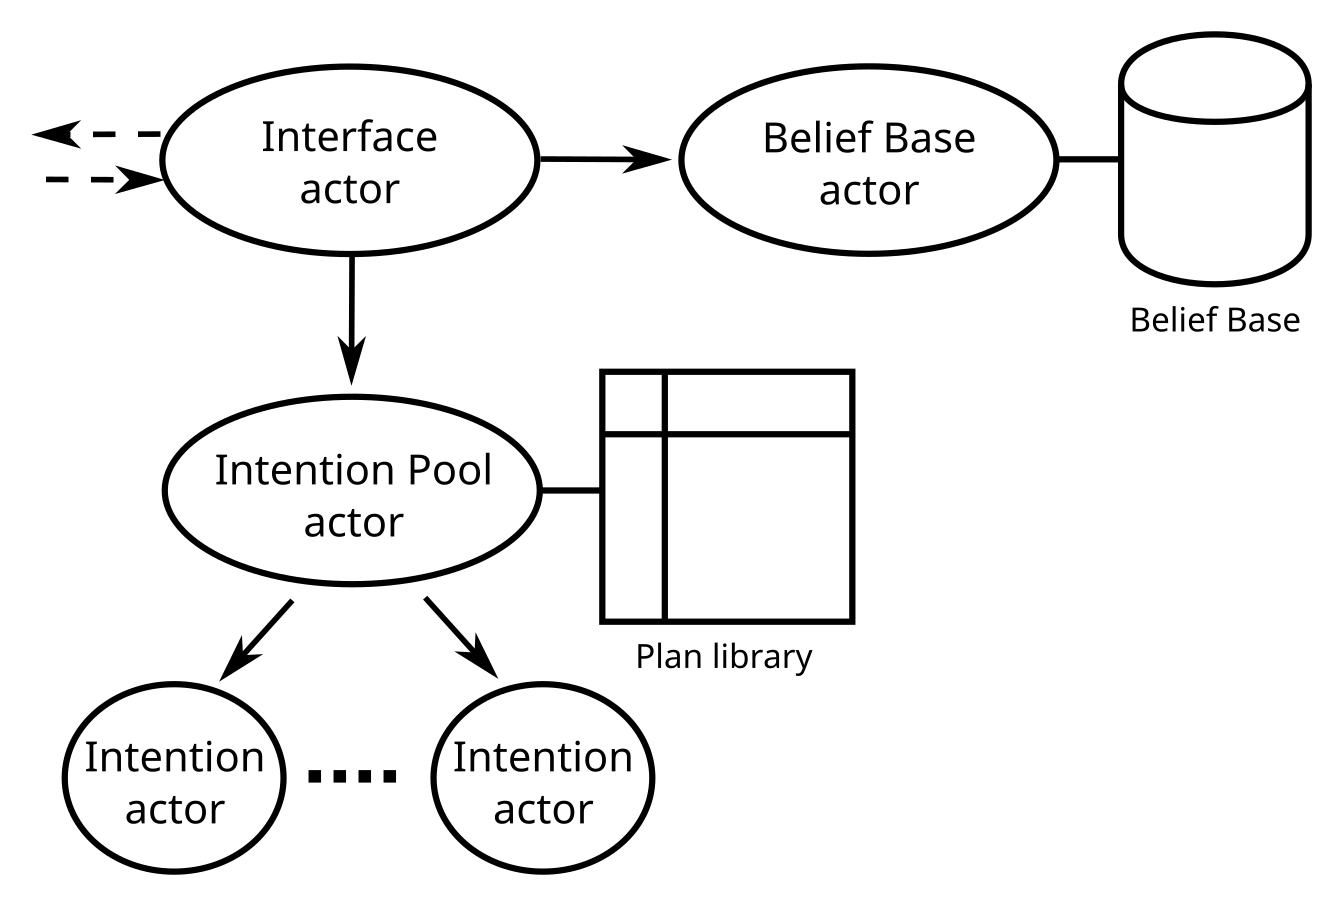
\includegraphics[width=0.5\linewidth]{arch3.png}
%   \caption{AgentScriptCC execution architecture}
%   \label{fig:asc2}
%   %\Description{Actor-based architecture of an agent}
% \end{figure}


\subsection{Testing Approach\label{sec:testing-approach}}

%There have been multiple works about testing Agent-Oriented Programming Languages \cite{Winikoff2016} which typically approach the tested entity, i.e the agent program from the higher level cognitive perspective trying to take into account the complex inner workings an agent may have. While this may be a necessity for advancement of the AOP field, in practice without integration with modern software testing approaches, the AOP frameworks can not take advantage of many testing tools developed by the respective community.

% What can an agent or MAS designer use testing libraries or services mainly built for other programming paradigms?

In a typical \textit{unit} or \textit{integration test} of a computational entity under test (e.g. a class, a web service), the designer sets up an initial setting (e.g. one or multiple object instances, web services, a client), and then, based on certain invocations (e.g. function calls, access/service requests), a set of \textit{assertions} are checked to verify the internal state, or some observable behavior of the tested entity, or its effect on the environment (e.g. function results, service responses, modifications of other entities). 

Internal attributes (of objects or services) are generally harder to access and therefore to verify. Best practices of Test-Driven Development (TDD) address this issue by means of \textit{Dependency Injection} (DI): the dependencies of each entity should be instantiated from outside the entity and then passed to it e.g. as parameters (typically to the class constructor in object-oriented programming). %, in terms of Object Oriented Programming this would mean instantiating the objects that a class depends on in the outer scope and passing these objects to the class constructor as parameters.
This allows the tester to isolate and observe the internal mechanisms of the entity under test by using ``mocked'' dependencies. 
To enhance testability, multiple components of ASC2 agents, including their belief base and communications layer, are injected as external dependencies.

In any certain situation, we can look at a single agent or multiple agents (a MAS) as a computational entity under test, and this entity has also a set of internal attributes, observable behavior, and possible interactions with its environment. The single agent or multiple agents under test can be instantiated from one or more scripts. The setting could include any other types of entities e.g. other possibly mocked agents, external objects, etc. The initial state of the agent(s) and of the other related entities defines the initial setting of the test, the invocation/probing action of a test suite is typically a series of messages sent to the agents. The expected effect(s), behavior(s) or state(s) of an entity rely heavily on the entity under test. For a small system including one or only a few agents, each message or the beliefs of the agent(s) may be needed to be verified, whereas in a complex system, the designer may only need to verify emergent pattern in the interactions of the agents or major shifts in the state of the system.

\begin{figure}[t!]
  \centering
  \hspace{-5pt}
  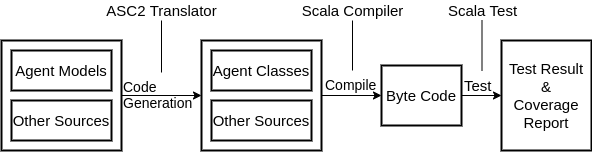
\includegraphics[width=0.80\linewidth]{ch_emas/sbt_proc.png}
  \caption{Compile/Test process of an ASC2 program with sbt}
  \label{fig:sbt1}
\end{figure}

In our approach, we aim to allow the designer to utilize any off-the-shelf testing tool (library, service, etc.) directly into their development chain, even more so to enable the designer to test their program via any standard build chain. 
In the case of the ASC2 framework, its current implementation is based on Scala, and we considered as target build tool \textit{sbt}\footnote{\url{https://scala-sbt.org/}}, which enables us to also use JVM/Scala testing libraries like \textit{JUnit} or \textit{ScalaTest}. We have then developed a sbt plugin\footnote{\url{https://github.com/mostafamohajeri/sbt-scriptcc}} that %when enabled in a project
---as part of the compile task---iterates over the scripts written in AgentScript DSL in the project sources and uses the AgentScript Translator to generate Scala implementations of the agents. Code generation is a standard part of build tools like sbt or maven, therefore, the generated sources are also managed by the build tool and are immediately available to rest of the project. The general overview of the \textit{Compile/Test} cycle of an agent-based system developed via ASC2 and built by sbt is presented in figure \ref{fig:sbt1}. Note that this process is fully automated by sbt. 


A MAS of this type can be started in two ways. After bootstrapping it as an empty instance of the MAS infrastructure, the designer can either use configuration files (e.g. JSON) to specify the agents of the system or alternatively, use lower-level code (e.g. Scala/Java) to manually spawn agents via their respective class in the generated code. In this work, we preferred the latter approach, as it provides better control over the test scenarios.

To complete our Compile/Test process, in addition to the \textit{ScalaTest} library, we also used the \textit{Akka Testing} library: at run-time, ASC2 agents are essentially Akka actor micro-systems and this library provides many convenient tools for testing actors. Both libraries are used out of the box and no modifications have been done to adapt them to the framework. With this configuration, each scenario to be verified can the written as a test suite in ScalaTest to test whether one or multiple agents behave as expected.

\begin{listing}[!tb]

\centering
\begin{tcolorbox}[left=2pt,right=2pt,top=2pt,bottom=2pt,arc=0pt,
                  boxrule=0pt,toprule=1pt,
                  colback=white]
\begin{minted}[linenos]{prolog}
+!init(W) : W > 1 =>
    Nbr = "worker" + 
        ((#name.replaceAll("worker","").toInt mod W) + 1);
    +neighbor(Nbr).

+!token(0) =>
    #coms.achieve("master", done).

+!token(N) : neighbor(Nbr) =>
    #coms.achieve(Nbr, token(N - 1)).
\end{minted}
\end{tcolorbox}
    \caption{Token ring \texttt{worker} script in AgentScript DSL}
    \label{lst:script_1}

\end{listing}

\section{Illustrative Example}
\label{sec:example}
To illustrate an application of our testing approach we consider a MAS constructed around a Token Ring system, commonly used in both distributed systems and MAS \cite{MohajeriParizi2020,Cardoso2013}. This system consists of one master agent and $W$ worker agents; at the start of the program the master sends an $init(W)$ message to all worker agents to inform them of the total number of the workers in the ring, each worker upon receiving this message finds its neighbor, forming a closed ring. Then, $T$ tokens are distributed among the workers, each token has to be passed $N$ times in the ring formed by workers. When all $T$ tokens have been passed $N$ times and this was reported to the master, the program ends.

% \begin{comment}

% A token ring MAS program should:
% \begin{itemize}
%     \item create one master and $W$ number of workers;
%     \item the master sends a $init(W)$ event to all workers, where $W$ is the number of workers in the ring; then it distributes all the tokens $1\leq i \leq T$ with a counter $N$ to workers;
%     \item each worker that receives $init(W)$ should determine its neighbor in order to form and to complete its ring;
%     \item when a worker receives a token it subtracts from the token's counter and sends it to its neighbor unless the token's counter has reached $0$ in which case it sends a $done$ message to the master;
%     \item the program finishes when all $T$ tokens have been passed listing $N$ times and the master have received $T$ number of $done$ messages
%  \end{itemize}
 
%  \end{comment}

\subsection{Unit/Agent Testing}
We will focus in particular on the script of the worker agents shown in listing \ref{lst:script_1}. We perform the tests taking the standpoint of a \textit{whitebox} test engineer, meaning that we test the script of the agent knowing its internal workings; nevertheless, the tests are still performed externally, we do not modify the script in order to test it\footnote{\url{https://github.com/mostafamohajeri/agentscript-test}}.

\subsubsection{Testing Successful Scenarios}
By viewing the script in listing \ref{lst:script_1}, we can see that the agent has a total of 3 plans for 2 separate goals. Theoretically, we need at least 3 tests to cover the successful execution of all the plans. However, while the success criteria for plans is simple (completion of execution), achievements of goals can be more complicated and the testing framework needs to provide the flexibility to define them. The success criteria for the \texttt{init(W)} and \texttt{token(N)} goals are quite different. In the latter the expected behaviour in both plans is an observable event, i.e. a certain \texttt{achieve} message sent by the agent to another specific agent. In the former case there is no observable behavior and the success criterion is a specific update of the agent's belief base.





\begin{listing}[!tb]
\centering
\begin{tcolorbox}[left=2pt,right=2pt,top=2pt,bottom=2pt,arc=0pt,
                  boxrule=0pt,toprule=1pt,
                  colback=white]
\begin{minted}[fontsize=\small,linenos]{scala}
class TokenRingWorkerSpec extends ... {

  val mas = new MAS()
  val verifiableBB  = new BeliefBase()
  val mockedMaster = testKit.createTestProbe[IMessage]()
  val mockedNeighbor = testKit.createTestProbe[IMessage]()
  val worker

  override def beforeAll(): Unit = {
    mas.registerAgent(new worker(bb = verifiableBB), name = "worker1")
    mas.registerAgent(mockedMaster, name = "master")
    mas.registerAgent(mockedNeighbor, name = "worker2")
    worker = mas.getAgent("worker1")
  }

  "A worker agent" should {
    "have its neighbor in its belief base after `!init(N)`" in {
      worker.event(achieve,"init(50)").send()
      mockedMaster.expect(GoalAchievedMessage())
      assert(verifiableBB.query("neighbor(worker2)") == true)
    }

    "send a `!done` to master on `!token(0)`" in {
      worker.event(achieve,"token(0)").send()
      mockedMaster.expect(event(achieve,"done").source(worker))
    }

    "send a `!token(N-1)` to its neighbor on `!token(N)`" in {
      worker.event(achieve,"token(10)").send()
      mockedNeighbor.expect(event(achieve,"token(9)").source(worker))
    }
  }
}
\end{minted}
\end{tcolorbox}
    \caption{Test suite for the \texttt{worker} agent}
    \label{lst:test_1}
\end{listing}

The test specification we used for the worker agent can be seen in listing \ref{lst:test_1}. In line 3 an empty MAS object is created. The criterion of success for \texttt{init(W)} plan depends on the agent's beliefs, therefore we need to be able to verify the internal state of agent's belief base. First we create an instance of \texttt{BeliefBase} class (line 4) and when the agent under test (\texttt{worker1}) is being instantiated (line 10), this object is injected in the agent as its belief base; with this approach at any point in the tests we can simply access the agent's beliefs to query them for verification purposes or even modify the agent's belief base for setting up test scenario states.

Only one agent (\texttt{worker1}) is under test and the other agents present in the suite can be mocked. As ASC2 agents are actor micro-systems, an agent can be mocked by a single actor. In lines 5 and 6, two \textit{probe} actors are created to be the stand-ins for the master agent and (\texttt{worker1})'s neighbor in the tests and they are then registered to the system (lines 11 and 12). This type of mocking gives us the ability to verify all the interactions that the agent under test may have had with these probe actors.

%Note that ScalaTest (or any other testing tool) already provides convenient interface functions like \texttt{beforeAll} to set up a test.

The rest of the test suite contains 3 tests, in the first test in line 18 a goal event \texttt{init(50)} is sent to the \texttt{worker1} agent and it is expected that after this goal is achieved (line 19), the belief base of the agent contains the belief defined by the term \texttt{neighbor(worker2)} which is verified in line 20. In the next test, a goal message \texttt{token(0)} is sent to the agent (line 24) and then it is verified that the agent sends a \texttt{done} message to the master (line 25). The final test follows the same pattern by sending a goal message \texttt{token(10)} (line 30) and the verification includes a \texttt{token(10-1)} message to its neighbor (line 30). Note that in all the tests, the messages sent to the \texttt{worker1} agent do not specify any source, this is because in the script in listing \ref{lst:script_1}, the source of the messages is not checked meaning it is not necessary to specify the source. As these tests are written in a standard testing library, build tools such as \textit{sbt} can execute them in their build chain. By running the tests in the sbt shell we are able to see the output presented in listing \ref{lst:result_1} that indicates our program has passed this test.

\begin{listing}[!h]
\begin{Verbatim}[fontsize=\small]
[info] A worker agent should
[info] - have its neighbor in its belief base after `!init(N)`
[info] - send a `!done` to master on `!token(0)`
[info] - send a `!token(N-1)` to its neighbor on `!token(N)`
...
[info] All tests passed.
\end{Verbatim}
\vspace{-5pt}
    \caption{Output of the \texttt{worker} agent test suite}
    \label{lst:result_1}
\vspace{-5pt}
\end{listing}




\subsubsection{Testing Failure Scenarios}
Successful executions are only a part of the full story. Indeed, in software testing it is acknowledged that covering \textit{failures} is both more important and challenging, and thus requires more critical thinking by the test engineer \cite{ArtOfTesting}. Interestingly, failure tests are especially important in agent-based programming because failing under certain conditions may sometimes be the correct behavior for an agent. 

Two failure tests are presented in listing \ref{lst:test_2}. The first test sends a \texttt{init(W)} goal message to the agent with \texttt{W=-1} (line 3) but the first plan is applicable only for \texttt{W > 1} and the expected behavior of the agent in this situation is a failure which is verified by expecting a \texttt{NoApplicablePlan} message. In the second test, a goal message \texttt{unknown} is sent to the agent (line 8) for which the agent does not have any plans and it should reply with a \texttt{NoRelevantPlan} (line 9). Note that failure of a goal is not only reflected by the absence of an applicable plan or more generally failure in execution of a plan; similar to the success scenarios, the designer can define any other arbitrary criteria for a failure scenario.

\begin{listing}[!tb]
\centering
\begin{minted}[linenos]{scala}
"A worker agent" should {
  "send a `NoApplicablePlan()` on `!init(-1)`" in {
    worker.event(achieve,"init(-1)").source(mockedMaster).send()
    mockedMaster.expect(NoApplicablePlan())
  } 
  
  "send a `NoRelevantPlan()` on `!unknown`" in {
    worker.event(achieve,"unknown").source(mockedMaster).send()
    mockedMaster.expect(NoRelevantPlan())
  }
}
\end{minted}
\vspace{-5pt}
    \caption{Failure tests for \texttt{worker} agent}
    \label{lst:test_2}
\vspace{-5pt}
\end{listing}

% This type of failure test, despite being simple, can be a very powerful tool for the designer to reveal the incorrect behaviors of the agent program.

Although we acknowledge that testing an agent program for every possible failure can easily become an infeasible task \cite{Winikoff2015,Winikoff2017}, certain failures may be particular important for the designer to test, therefore there is value in enabling this possibility.

\subsection{Coverage}

% Continuing from the previous section on how we use off-the-shelf testing libraries to write tests for ASC, 

We explore at this point whether and how off-the-shelf coverage tools such as \textit{scoverage}\footnote{\url{http://scoverage.org/}} can be used for code coverage analysis of agent programs written in ASC2, considering both statement and branch coverage aspect. To perform this we simply add the scoverage plugin to our project and generate a coverage report.

The coverage report produced for the worker agent by means of the previous tests is presented in Table \ref{tab:coverage}. The \texttt{worker.Agent} row shows the coverage for the internal mechanisms of the agent, like e.g. \textit{event handling}, 
%(excluding the belief base) 
while the other rows show the coverage report for each separate event, as an example, the \texttt{worker.token\_1} refers to an event \texttt{token} in \texttt{worker} agent with 1 parameter. The branch coverage report mainly concerns conditional statements in the generated Scala code of the agent and should be regarded only as informal information about the coverage of the main script.

These results show that our tests indeed covered most of the behaviors that the agent might have. In fact, by exploring the coverage analysis we can see the reason for which the \texttt{worker.token\_1} has less coverage: the missed branch can be explained by the fact that the tests did not include any scenario in which the \texttt{token(N)} plan fails. Also note that while the example script did not contain any sub-goals or conditional statements in the plans, ASC2 Translator generates sub-goal adoptions as function calls and translates conditional statements to their counterpart in the underlying language, therefore, coverage tools like \textit{scoverage} are able to calculate the correct number of covered and total possible branches for deeper goal-plan trees.
\vspace{-5pt}

\setlength{\tabcolsep}{0.5em} % for the horizontal padding
{\renewcommand{\arraystretch}{1.1}% for the vertical padding
\begin{table}
    \centering
    \begin{tabular}{lll}
        \toprule
        Component &  Statement Coverage \% & Branch Coverage (Covered/Total) \\
        \midrule
       \texttt{worker.Agent}  &  93.5  & 6/6 \\
       \texttt{worker.init\_1} &  93.5  & 2/2 \\
       \texttt{worker.token\_1} &  80.2  & 3/4 \\ \bottomrule
    \end{tabular}
    \vspace{5pt}
    \caption{Coverage analysis of the \texttt{worker} agent}
    \label{tab:coverage}
    \vspace{-10pt}
\end{table}
}

\subsection{Integration/System Testing}
%Integration testing refers to the activity of verifying that different modules of a software system work together in a correct way. In practice, software integration tests often are done on modules developed by different teams located in different repositories and it is important that testing tools support this type of setups. Furthermore, in the MAS testing community there are conceptual guidelines on how to decide what the modules of a systems are \cite{Moreno2009}. We continue with an integration test setting that aligns the theoretical aspect of MAS testing with the practical requirements of software testing.

%The integration test suite that verifies a system consisting of the previously mentioned \texttt{worker} agent hosted on one repository and a \texttt{master} agent hosted on another. The integration test project will need to fetch both projects prior to running the test suite.  

%The MAS testing community provides conceptual guidelines on how to decide what the modules of a systems are \cite{Moreno2009}. We will follow these guidelines for giving an example of integration test suite,

Even following the guidelines on categorizing different levels of testing in MAS \cite{Moreno2009}, there is no definite technical distinction in place. Typically test libraries provide mechanisms such as annotations for the designer to label test suites with its (their) related level(s) to orchestrate their execution. As illustration, we consider an integration test to verify a token ring MAS system consisting of the previously mentioned \texttt{worker} agents and a \texttt{master} agent. The test suite is reported in listing \ref{lst:test_3}.

\begin{listing}[!tbh]
\centering
\begin{minted}[fontsize=\small,linenos]{scala}
class TokenRingIntegrationSpec extends ... {
  
  //a communication layer that records a trace of the interactions
  object recordedComs extends AgentCommunicationsLayer { ... }

  val token_pattern = "token\\([0-9]+\\)".r
  val done_pattern = "done".r

  "A token ring MAS with W = 100, T = 50 and N = 4" should {
    "have 250 `token(X)` and 50 `done` message" in {
      // create the agents
      mas.registerAgent(new worker(coms = recordedComs), num = 100)
      mas.registerAgent(new master(coms = recordedComs), name = "master")
      // invoke the system
      mas.getAgent("master").event(achieve, "start(50,4)").send()
      // verify the interactions
      watchdog.expectTerminated( mas, 10.seconds )
      assert(recordedComs.trace.count(token_pattern.matches) == 250)
      assert(recordedComs.trace.count(done_pattern.matches) == 50)
    }
  }
}
\end{minted}
\vspace{-5pt}
    \caption{Integration test suite for the token ring system}
    \label{lst:test_3}
    \vspace{-5pt}
\end{listing}


The test will be centered around the interactions between agents and the state of the system in a specific setting of our token ring. The token ring is defined with 100 \texttt{worker} agents and 1 \texttt{master} agent (lines 12-13), and, to be able to verify the exhibited interactions, we use dependency injection to initialize all the agents by means of an overridden instance of the communication layer (line 4), created to record every message passed in the system into a list. 

To invoke the system, a \texttt{start(T,N)} is sent to the \texttt{master} agent (line 15). We are interacting with the \texttt{master} from a \textit{black box} perspective: although the event \texttt{start(T,N)} is exposed, the internal mechanisms of this agent are assumed to be unknown.

Three criteria are verified for this system. Firstly, we consider a system level performance based criteria as we expect the system to be terminated under 10 seconds (line 17). Next, we use two known expectations from a token ring system to verify the correct execution of the system: at the end of execution, there should be (a) $T$ number of \texttt{done} messages and (b) $T \times (N + 1)$ number of \texttt{token(X)} messages in the trace. The interaction verification statements are presented respectively in lines 18-19. Recalling the flexible definitions of testing levels, note that these integration/system test could be considered from the perspective of \texttt{master} agent as a unit/agent level test possibly with mocking the \texttt{worker} agents. Similar to previous tests, running this suite via sbt yields the output in listing \ref{lst:result_2}.

\begin{listing}[!h]\vspace{-10pt}
\begin{Verbatim}[fontsize=\small]
[info] A token ring MAS with W = 100, T = 50 and N = 4 should
[info] - have 250 `token(X)` and 50 `done` message
...
[info] All tests passed.
\end{Verbatim}
\vspace{-5pt}
    \caption{Output of the token ring integration test suite}
    \label{lst:result_2}
\end{listing}


\vspace{-20pt}
\subsection{Continuous Integration}
The proposed approach for testing can be easily combined with online CI services. This process generally includes utilizing source repositories like Github\footnote{\url{https://github.com/}}, CI services like TravisCI and code analysis services like Coveralls\footnote{\url{https://coveralls.io/}}. The only step needed to set  the CI cycle for an ASC2 project is to configure the source repository of the project in a way that the automated CI cycle is triggered on every \texttt{push} to the repository. This can be done by adding a configuration file that provides information for the CI service how to compile and test the project via sbt.%, and on how to register the project on the relevant CI service. 

Following this method, a MAS project does not need to be only located in a single source repository. For instance, different types of agents can be developed in different projects by separate teams and only be used as dependencies in the development of the system. We believe this is an interesting practical innovation, improving the scalability of MAS projects with respect to their development. 


An overview of an example CI process for the token ring is presented in Figure \ref{fig:ci} in which the sources of \texttt{worker} and \texttt{master} agents are located in separate repositories, and a third token ring repository uses them as dependencies. When the system designer pushes the project to the repository, the CI service fetches the source and compiles and tests it via sbt and records the results\footnote{\url{https://travis-ci.com/github/mostafamohajeri/agentscript-test}}. Then, the code coverage report is committed to the code analysis service\footnote{\url{https://coveralls.io/github/mostafamohajeri/agentscript-test}}.


\begin{figure}[t!]
  \centering
  \hspace{-5pt}
  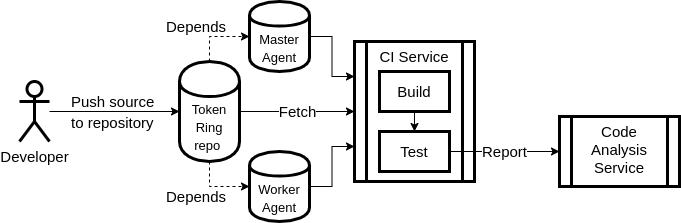
\includegraphics[width=1\linewidth]{ch_emas/ci.png}
  \caption{Continuous integration applied on a Token ring program whose master and worker agent scripts are located on other repositories.}
  \label{fig:ci}
  %\Description{Actor-based architecture of an agent}
\end{figure}

% AgentScript is JVM based so in principle MCAPL should work on it
% Test Generation can be done with this approach

\section{Discussion and Conclusion}
\label{sec:discussion}
%While the successful execution of the plans share the same criteria: completion without exceptions, for an intelligent agent the criteria for the achievement of the respective goals may be different and critically the testing approach for such agents allows for flexible definitions of success criteria.

Despite the critical points/observations concerning MAS testing raised in the literature, in this chapter we % break a lance 
provide several support arguments for using  mainstream testing tools for MAS and agent-based programming, by means of a concrete use case. We implemented a multi-agent system reproducing a token ring benchmark with the framework ASC2, and then we run tests (success, failure, coverage) at unit/agent level as well as at integration/system level. 

%The bottom-line about the applicability of such a method is that the used agent and MAS programming framework needs to be compatible with mainstream software build processes. By satisfying this requirement (as in the case of ASC2), one can utilize development tools and services available to other programming languages for testing, coverage analysis and CI. Our experience in attempting to integrate agent-based development with concurrent development conducted by other programming methods in the context of data-sharing infrastructures made us clear the necessity and urgency of this innovation. We do not claim here that all application domains of MAS require such an operational constraint, but we observe that there are applicative niches that can greatly benefit of  cross-compilation solutions.



At the unit and agent level (unit testing) we performed tests concerning events, plans and goals. The somehow unexpected result of the experiment is that such an approach does not neglect the theoretical complexity of BDI agents but it truly offers a complementary tool for their development. We were able to test successful (plan) completions, internal states and the belief base, failures, and fine-grained interactions. 
These possibilities can be seen as offering  constructs mapping e.g. to declarative and procedural goals in BDI agents \cite{Winikoff2002}: the designer can define the achievement/failure of a goal not only in terms of completion/exception of a plan, but also as determined by any arbitrary indicator internal or external to the agent. This showed that testability of agent programs defined in a framework is closely related to the design choices of that framework. 
% t 

At the integration/group and system/society level (integration testing) we performed tests with simple verification criteria, but these criteria can easily be extended to more sophisticated and realistic interaction analysis and verification methods developed by the MAS community \cite{Botia2006}. Additionally, we illustrated how the proposed approach enables the MAS designer to take advantage of continuous integration (CI) services without extra effort. This is particularly important for MAS designers that require to integrate and test their work continuously with other projects.

There is an additional benefit of using mainstream test tools for BDI agents, and especially for frameworks that are based on higher-level logic-based DSLs. Those frameworks generally map primitive actions to constructs specified in a lower-level programming language like Java. By using a testing process compatible with both higher level models and lower level implementations, the testing process can be more efficient and seamless for the designer specially if the agent models are only a part of a project that includes other computational entities that are being developed alongside the agents. 

An issue in using mainstream test libraries for a BDI framework with a logic-based DSL is the disparity between the high-level agent DSL and the lower-level language used for the tests. This can be addressed by either developing approaches to write tests in the high-level DSL or creating interfaces for the low-level language to enable the test engineer to implement tests at a proper level of abstraction. In this work we have taken the latter approach.
%In this work we used the ASC2 agent programming framework to present our approach, 
The intuition behind this choice was that frameworks based on cross-compila-tion \cite{Astra,Sarl} produce source codes that can be directly integrated within standard build tools.

Can our results be generalized to other agent programming frameworks?
Motivated by the success of works like AJPF/MCAPL \cite{Dennis2016} that provides model checking for multiple BDI frameworks, as a future study we intend to explore how to apply this approach to a wider range of MAS frameworks.
Yet, we can already trace some higher-level considerations.
%This raises the question:
The answer, at the unit/agent level, depends on compilation and the execution model of those frameworks. For frameworks like Jade and JS-son \cite{Kampik2020}, that use mainstream programming languages to define agents, these tools should be compatible out of the box with minor effort \cite{Khamis2013}. For cross-compilation-based frameworks like Astra \cite{Astra} and ASC2 \cite{MohajeriParizi2020} it is only the matter of tooling (e.g. build tool plugins) to allow them to use mainstream testing tools. For interpreter-based frameworks like Jason \cite{Bordini2005} and GOAL \cite{Hindriks2009a}, because they require their own dedicated reasoning engines and execution environment, %which are not recognizable by the mainstream tools and developing tools to bridge them into mainstream testing tools
testing via such tools may prove to need more work and possibly modifications to the framework. This issue may be not so problematic, as there are already many works that propose dedicated testing and debugging approaches for interpreter-based frameworks \cite{Koeman2016}.
%be impractical and 
%however, typically interpreter-based frameworks provide their own dedicated testing/debugging approaches \cite{Koeman2016}.

At the integration and system level, and also with respect to compatibility with CI services, generally externalized to the execution of the tested entity, we believe it is possible to consolidate other frameworks regardless of their compile/interpret model. This could lead to seamless integration testing of systems defined in each framework with mainstream software testing tools or dedicated ones.

In perspective, our overarching research concerns socio-technical and complex multi-domain infrastructures; we believe that Agent-Oriented Software Engineering can be a powerful technical tool with robust theoretical foundations for designing, modelling, implementing and testing such systems.  Enhancing their development cycle goes with a seamless integration of multi-agent systems into modern infrastructures. This is a critical requirement to utilize the full potential of MAS in a real production-level setting. 
